% 1989 年上海卷第五题解答图：圆盘与直线 x-y=3 的交集线段
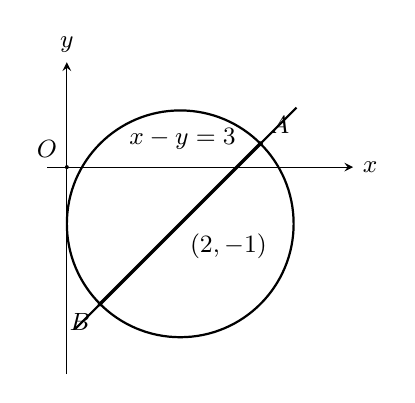
\begin{tikzpicture}[scale=0.72,>=stealth,font=\small]
  \draw[->] (-0.35,0)--(5.05,0) node[right] {$x$};
  \draw[->] (0,-3.65)--(0,1.85) node[above] {$y$};
  \draw[thick] (2,-1) circle[radius=2];
  \draw[thick] (0.15,-2.85)--(4.05,1.05);
  \draw[very thick] (2-1.41421356,-1-1.41421356)--(2+1.41421356,-1+1.41421356);
  \fill (0,0) circle (1pt) node[above left] {$O$};
  \fill (2+1.41421356,-1+1.41421356) circle (1.2pt)
    node[above right] {$A$};
  \fill (2-1.41421356,-1-1.41421356) circle (1.2pt)
    node[below left] {$B$};
  \node[below right] at (2,-1) {$(2,-1)$};
  \node[above left] at (3.15,0.15) {$x-y=3$};
\end{tikzpicture}
